\documentclass{article}
\usepackage[margin=1in]{geometry} % Please keep the margins at 1.5 so that there is space for grader comments.
\usepackage{amsmath,amsthm,amssymb}
\usepackage[linesnumbered,ruled,vlined]{algorithm2e}
\usepackage{graphicx}
\usepackage{caption}
\usepackage{subcaption}

\graphicspath{ {./code/weighted_logistic_reg/} }



\newcommand{\R}{\mathbb{R}}
\newcommand{\Z}{\mathbb{Z}}
\newcommand{\N}{\mathbb{N}}
\newcommand{\Q}{\mathbb{Q}}
\newcommand{\QED}{\textbf{QED}}

\newenvironment{theorem}[2][Theorem]{\begin{trivlist}
\item[\hskip \labelsep {\bfseries #1}\hskip \labelsep {\bfseries #2.}]}{\end{trivlist}}
\newenvironment{lemma}[2][Lemma]{\begin{trivlist}
\item[\hskip \labelsep {\bfseries #1}\hskip \labelsep {\bfseries #2.}]}{\end{trivlist}}
\newenvironment{claim}[2][Claim]{\begin{trivlist}
\item[\hskip \labelsep {\bfseries #1}\hskip \labelsep {\bfseries #2.}]}{\end{trivlist}}
\newenvironment{problem}[2][Problem]{\begin{trivlist}
\item[\hskip \labelsep {\bfseries #1}\hskip \labelsep {\bfseries #2.}]}{\end{trivlist}}
\newenvironment{proposition}[2][Proposition]{\begin{trivlist}
\item[\hskip \labelsep {\bfseries #1}\hskip \labelsep {\bfseries #2.}]}{\end{trivlist}}
\newenvironment{corollary}[2][Corollary]{\begin{trivlist}
\item[\hskip \labelsep {\bfseries #1}\hskip \labelsep {\bfseries #2.}]}{\end{trivlist}}

\newenvironment{solution}{\begin{proof}[Solution]}{\end{proof}}

\begin{document}

\large % please keep the text at this size for ease of reading.
\linespread{1.5} % please keep 1.5 line spacing so that there is space for grader comments.

% ------------------------------------------ %
%                 START HERE             %
% ------------------------------------------ %

{\Large Problem Set {1}% Replace with appropriate number -- keep this THE SAME even when you revise and resubmit.
\hfill  sz CS 229}

\vspace{0.5in}

% -----------------------------------------------------
% The following two environments (claim, proof) are
% where you will enter the statement and proof of your
% first problem for this assignment.
%
% In the theorem environment, you can replace the word
% "theorem" in the \begin and \end commands with
% "theorem", "proposition", "lemma", etc., depending on
% what you are proving.
% -----------------------------------------------------


% Question 1
{\large \bf Q1 Newton's method for computing least squares}\\
Prove that if we use Newton's method to solve the least squares optimization problem, 
then we only need one iteration to converge to \(\theta^*\).\\
a. Find the Hessian of the cost function \(J(\theta) = \frac{1}{2} \sum^{m}_{i=1}(\theta^{T}x^{(i)}-y^{(i)})^2\).\\
\\
We know that
\begin{equation*}
  \begin{aligned}[c]
    \theta^T = \begin{bmatrix}
        \theta_0  &\theta_1  & \cdots   & \theta_d \\
        \end{bmatrix} \\
  \end{aligned}
  \qquad
  \begin{aligned}[c]
    x = \begin{bmatrix}
     x_0^{(i)} \\
     x_1^{(i)} \\
     \vdots   \\
     x_d^{(i)} \\
    \end{bmatrix}
    \text{where }\forall i, \quad x_{0}^{i} = 1
  \end{aligned}
\end{equation*}
Then each entry at index \(i,j\) of the Hessian is:
\begin{align*}
    H_{ij}(J(\theta)) & = \frac{\partial }{\partial \theta_{i} \partial \theta_{j}}
    \frac{1}{2}\sum^{m}_{k=1}(\theta^{T}x^{(k)}-y^{(k)})^2\\
    & = \frac{\partial }{\partial \theta_{j}} \sum^{m}_{k=1}(\theta^{T}x^{(k)}-y^{(k)})x_{i}^{(k)}\\
    & = \frac{\partial }{\partial \theta_{j}} \sum^m_{k=1}(\theta_0^{(k)}x_{0}^{(k)}x_{i}^{(k)}
        + \cdots + \theta_d^{(k)}x_{d}^{(k)}x_{i}^{(k)}-y^{(k)}x_{i}^{(k)})\\
    & = \sum^{m}_{k=1}(x_{i}^{(k)}x_{j}^{(k)})\\
\end{align*}
Thus
\[
    H = \begin{bmatrix}
        \sum_{k=1}^{m}x_{0}^{(k)}x_{0}^{(k)} & \sum_{k=1}^{m}x_{0}^{(k)}x_{1}^{(k)} & \cdots & \sum_{k=1}^{m}x_{0}^{(k)}x_{d}^{(k)} \\
        \sum_{k=1}^{m}x_{1}^{(k)}x_{0}^{(k)} & \sum_{k=1}^{m}x_{1}^{(k)}x_{1}^{(k)} & \cdots & \sum_{k=1}^{m}x_{1}^{(k)}x_{d}^{(k)} \\
        \vdots & \vdots & \ddots & \vdots \\
        \sum_{k=1}^{m}x_{d}^{(k)}x_{0}^{(k)} & \sum_{k=1}^{m}x_{d}^{(k)}x_{1}^{(k)} & \cdots & \sum_{k=1}^{m}x_{d}^{(k)}x_{d}^{(k)}
    \end{bmatrix} = X^T X
\]
where
\[
    X = \begin{bmatrix} \vec{x}^{(1)} \\ \vec{x}^{(2)} \\ \vdots \\ \vec{x}^{(m)} \end{bmatrix}
\]
\\\\
b. Show that the first iteration of Newton's method gives us the optimal solution to least squares problem.\\
Newton's method: \(\theta := \theta - H^{-1} \nabla _{\theta}J(\theta)\) \\
It is known that \(\nabla _{\theta}J(\theta) = X^{T}X \theta - X^{T} \vec{y} \), then,
\begin{align*}
    \theta - H^{-1} \nabla _{\theta}J(\theta) = & \theta - (X^{T}X)^{-1}(X^{T}X\theta - X^{T} \vec{y}) \\
    = & \theta - (X^{T}X)^{-1}X^{T}X\theta + (X^{T}X)^{-1}X^{T} \vec{y}\\
    = & \theta - \theta +   (X^{T}X)^{-1}X^{T} \vec{y}\\
    = &  (X^{T}X)^{-1}X^{T} \vec{y}\\
\end{align*} 
which is the optimal solution to the least squares problem. \\
\clearpage
{\large \bf Q2 Locally-weighted Logistic regression}\\
Implement the Newton-Raphson algorithm for optimizing \(\ell(\theta)\), where \(\ell (\theta)\) is cost function for locally weighted logistic regression, for a new query point
\(x\), and use this to predict the class of \(x\). 
\begin{figure}[h]
    \centering
  
    \begin{subfigure}{0.3\textwidth}
      \centering
      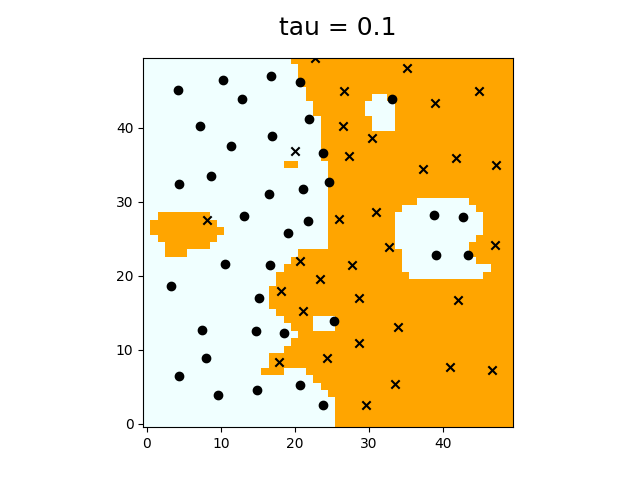
\includegraphics[width=\linewidth]{res_50_tau_0point1}
      \caption{Resolution = 50}
      \label{fig:subfig1}
    \end{subfigure}%
    \hfill
    \begin{subfigure}{0.3\textwidth}
      \centering
      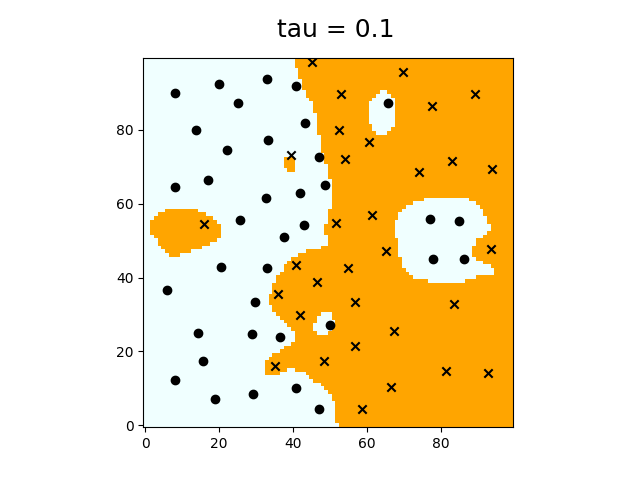
\includegraphics[width=\linewidth]{res_100_tau_0point1}
      \caption{Resolution = 100}
      \label{fig:subfig2}
    \end{subfigure}%
    \hfill
    \begin{subfigure}{0.3\textwidth}
      \centering
      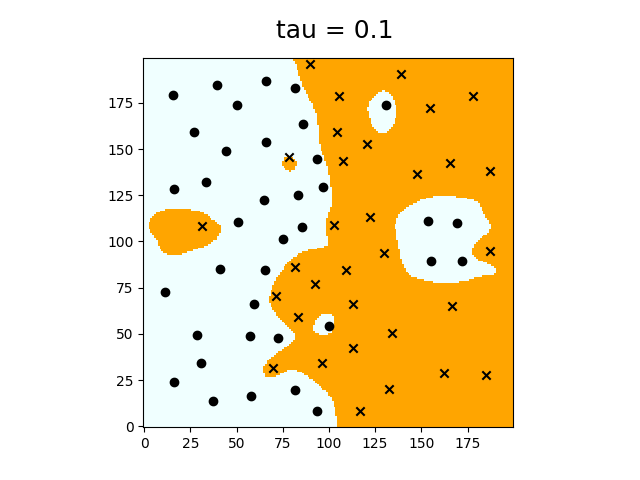
\includegraphics[width=\linewidth]{res_200_tau_0point1}
      \caption{Resolution = 200}
      \label{fig:subfig3}
    \end{subfigure}
  
    \caption{Results when varying the resolution}
    \label{fig:overall}
\end{figure}
\begin{figure}[!htb]
    \center
    \begin{subfigure}{0.3\textwidth}
      \centering
      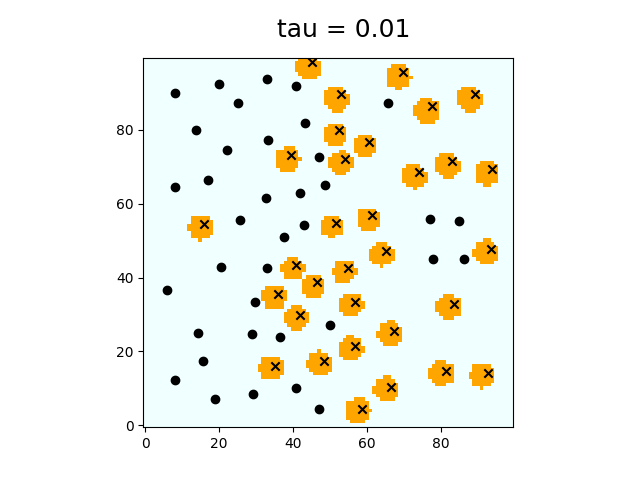
\includegraphics[width=\linewidth]{res_100_tau_0point01}
      \caption{Resolution = 100; \(\tau = 0.01\) }
      \label{fig:subfig4}
    \end{subfigure}%
    \hfill
    \begin{subfigure}{0.3\textwidth}
      \centering
      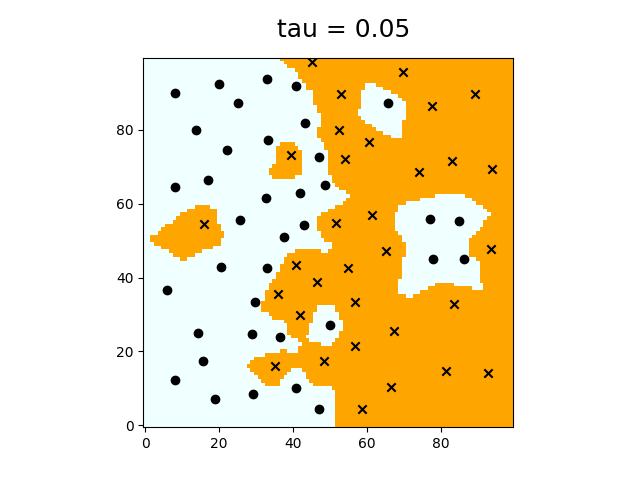
\includegraphics[width=\linewidth]{res_100_tau_0point05}
      \caption{Resolution = 100; \(\tau = 0.05\)  }
      \label{fig:subfig5}
    \end{subfigure}%
    \hfill
    \begin{subfigure}{0.3\textwidth}
      \centering
      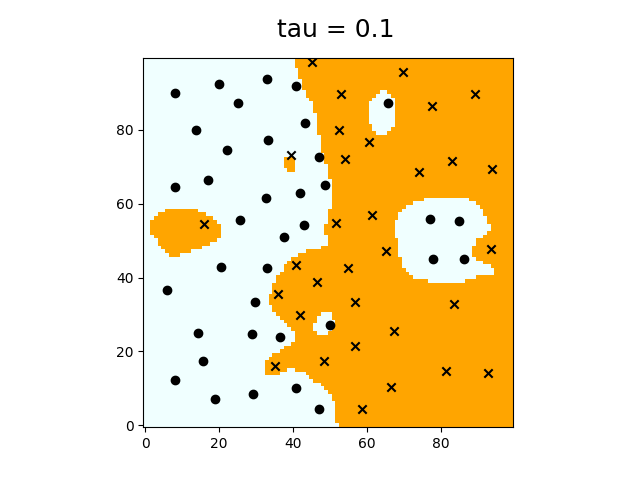
\includegraphics[width=\linewidth]{res_100_tau_0point1}
      \caption{Resolution = 100; \(\tau = 0.1\) }
      \label{fig:subfig6}
    \end{subfigure}

    \vspace{1cm}

    \begin{subfigure}{0.3\textwidth}
        \centering
        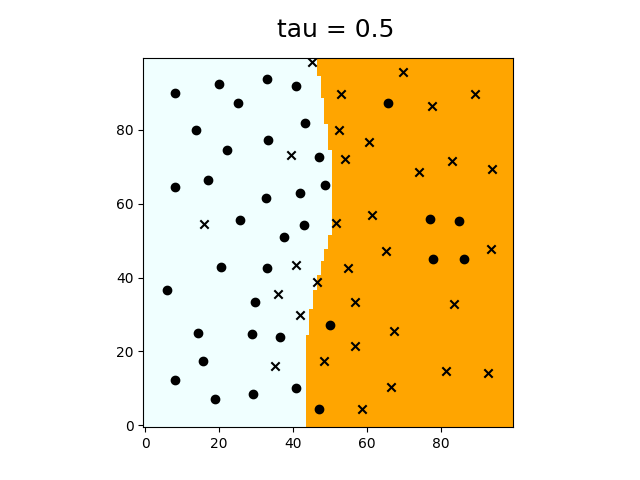
\includegraphics[width=\linewidth]{res_100_tau_0point5}
        \caption{Resolution = 100; \(\tau = 0.5\)  }
        \label{fig:subfig7}
      \end{subfigure}%
      \hfill
      \begin{subfigure}{0.3\textwidth}
        \centering
        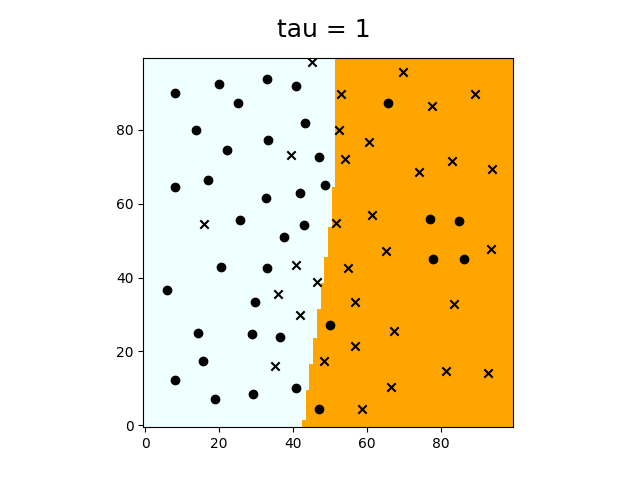
\includegraphics[width=\linewidth]{res_100_tau_1}
        \caption{Resolution = 100; \(\tau=1\) }
        \label{fig:subfig8}
      \end{subfigure}%
      \hfill
      \begin{subfigure}{0.3\textwidth}
        \centering
        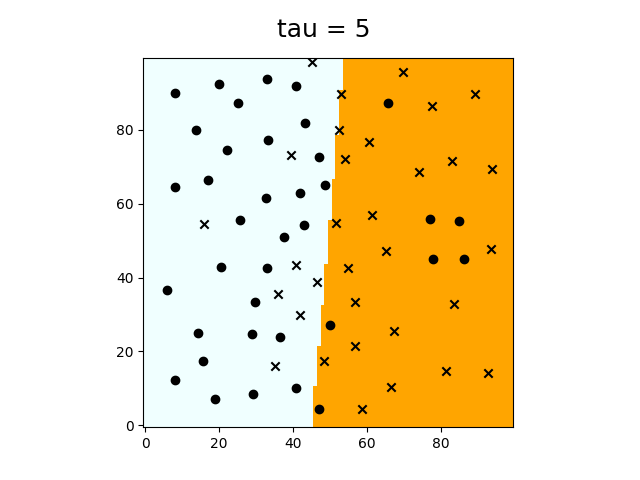
\includegraphics[width=\linewidth]{res_100_tau_5}
        \caption{Resolution = 100; \(\tau=5\) }
        \label{fig:subfig9}
      \end{subfigure}

  
    \caption{Varying \(\tau = 0.01, 0.05, 0.1, 0.5, 1, 5\) }
    \label{fig:overall2}
\end{figure}
\\
As we increase the bandwidth parameter \(\tau\), the decision 
boundary approaches a straight line. As \(\tau \to \infty\), the model
approaches an unweighted logistic regression model.
\clearpage
{\large \bf 3. Multivariate least squares}\\
a. Simplify to matrix-vector notation:
\[
    J(\Theta) = \frac{1}{2} \sum_{i=1}^{m} \sum_{j=1}^{p} ((\Theta^T x^{(i)})_j - y_j^{(i)})^2
\] 
where \(\Theta \in \R ^{n \times p} \).
\\ Let \(X = \begin{bmatrix}
 {x^{(1)}}^T \\
 {x^{(2)}}^T\\
  \vdots \\
  {x^{(m)}}^T \\
\end{bmatrix}\) , \(x^{(i)} \in \R^{n}\), and \(Y = \begin{bmatrix}
    {y^{(1)}}^T \\
    {y^{(2)}}^T\\
     \vdots \\
     {y^{(m)}}^T \\
\end{bmatrix}\), \(y^{(i)} \in \R^{p}\).
\\Let \(\Theta = \begin{bmatrix}
 \theta_1 & \theta_2 & \cdots  & \theta_p \\
\end{bmatrix}\), where \(\theta_i \in \R^n\).
\\
Then
\begin{align*}
    X\Theta - Y &= 
    \begin{bmatrix}
        x_{(1)}\cdot \theta_{1}-y^{(1)}_{1} & x_{(1)}\cdot \theta_{2}-y^{(1)}_{2} & \cdots & x_{(1)}\cdot \theta_{p}-y^{(1)}_{p} \\
        x_{(2)}\cdot \theta_{1}-y^{(2)}_{1} & x_{(2)}\cdot \theta_{2}-y^{(2)}_{2} & \cdots & x_{(2)}\cdot \theta_{p}-y^{(2)}_{p} \\
        \vdots & \vdots & \ddots & \vdots \\
        x_{(n)}\cdot \theta_{1}-y^{(m)}_{1} & x_{(m)}\cdot \theta_{2}-y^{(m)}_{2} & \cdots & x_{(m)}\cdot \theta_{p}-y^{(m)}_{p}
    \end{bmatrix} \\
    & = \begin{bmatrix}
     z_1 & z_2 & \cdots  & z_{p} \\
    \end{bmatrix}
\end{align*}

Notice that \(\frac{1}{2} \sum_{i=1}^{m} \sum_{j=1}^{p} ((\Theta^T x^{(i)})_j - y_j^{(i)})^2\) is equal 
to the sum of the square of every entry in \(X\Theta - Y\). We can calculate that by
taking the dot product of each column of \(X\Theta -Y\) by itself, then sum them up. 
First, 
\begin{align*}
    (X\Theta - Y)^T (X\Theta -Y) & = \begin{bmatrix}
        z_{1} \cdot z_{1} & z_{1} \cdot z_{2} & \cdots & z_{1} \cdot z_{p} \\
        z_{2} \cdot z_{1} & z_{2} \cdot z_{2} & \cdots & z_{2} \cdot z_{p} \\
        \vdots & \vdots & \ddots & \vdots \\
        z_{p} \cdot z_{1} & z_{p} \cdot z_{2} & \cdots & z_{p} \cdot z_{p}
    \end{bmatrix} \\
\end{align*}  
Thus
\[
    J(\Theta) = \frac{1}{2} \operatorname{tr}\{(X\Theta - Y)^T (X\Theta -Y)\}
\] 
Or 
\[
    J(\Theta) = \frac{1}{2} \operatorname{tr}\{(X\Theta - Y) (X\Theta -Y) ^ T\}
\]
\clearpage
b. Find the closed form solution for \(\Theta\) which minimizes \(J(\Theta)\).
\begin{align*}
    J(\Theta) & 
    = \frac{1}{2} \operatorname{tr} [(X\Theta - Y) (X\Theta - Y) ^ T] \\
    & = \frac{1}{2} \operatorname{tr}[(X\Theta - Y) (\Theta ^ T X^T - Y^T) ]\\
    & = \frac{1}{2 } \operatorname{tr}[X\Theta \Theta^{\mathrm{T}}X^{\mathrm{T}} - Y \Theta^{\mathrm{T}} X - X\Theta Y^{\mathrm{T}} + Y Y ^{\mathrm{T}}]\\
    & = \frac{1}{2} \{\operatorname{tr}[X\Theta\Theta^{\mathrm{T}}X^{\mathrm{T}} - \operatorname{tr}[Y\Theta^{\mathrm{T}}X^{\mathrm{T}}] - \operatorname{tr}[X\Theta Y^{\mathrm{T}}] + \operatorname{tr}[YY^{\mathrm{T}}]\}\\
\end{align*}

1.) Consider \(f = \operatorname{tr}[AXB]\) 
\begin{align*}
    f  = \sum_i [AXB]_{ii} 
    & = \sum_i \sum_j A_{ij} [XB]_{ji} \\
    & = \sum_i \sum_j A_{ij} \sum_k X_{jk} B_{ki}\\
    & = \sum_i \sum_j  \sum_k A_{ij} X_{jk} B_{ki}\\
    \therefore \frac{\partial f}{\partial X_{jk}} & = \sum_i A_{ij}B_{ki} =  \sum_i B_{ki} A_{ij} = [BA]_{kj}\\
    \therefore \frac{\partial \operatorname{tr}[AXB]}{\partial X} &= (BA) ^{\mathrm{T}} = A^{\mathrm{T}}B^{\mathrm{T}} && (1)\\
\end{align*}

2.) Consider \(f = \operatorname{tr}[AX^{\mathrm{T}}B]\)
\begin{align*}
    f & = \sum_i \sum_j \sum_k A_{ij}X_{kj} B_{ki}\\
    \frac{\partial f}{\partial X_{kj}} & = \sum_i A_{ij} B_{ki} = [BA]_{kj}\\
    \therefore \frac{\partial \operatorname{tr}[AX^{\mathrm{T}}B]}{\partial X} &= BA &&  (2)\\
\end{align*}
Now taking the partial derivatives with respect to \(X\) in each term of \(J(\Theta)\), 

\begin{align*}
    \frac{\partial \operatorname{tr}[X\Theta \Theta^{\mathrm{T}}X^{\mathrm{T}}]}{\partial \Theta} 
    & = \frac{\partial \operatorname{tr}[X\Theta A]}{\partial \Theta}  
    + \frac{\partial \operatorname{tr}[B\Theta^{\mathrm{T}}X^{\mathrm{T}}]}{\partial X}\\
    &\text{where \(A = \Theta^{T}X^T\) and \(\Theta\) is constant, and \(B = X\Theta\) where \(\Theta\) is constant.}\\
    & = (AX)^{\mathrm{T}} + X^{\mathrm{T}}B && \text{by (1) and (2)}\\
    & = X^{\mathrm{T}}X \Theta + X^{\mathrm{T}}X \Theta\\
    & = 2 X^{\mathrm{T}}X \Theta\\
    \frac{\partial \operatorname{tr}[Y\Theta ^{\mathrm{T}}X^{\mathrm{T}}]}{\partial \Theta}
    & = X^{\mathrm{T}}Y && \text{by (2)}\\
    \frac{\partial \operatorname{tr}[X\Theta Y^{\mathrm{T}}]}{\partial \Theta}
    & = (Y^{\mathrm{T}}X)^{\mathrm{T}} = X^{\mathrm{T}} Y && \text{by (1)}\\
    \frac{\partial \operatorname{tr}[YY^{\mathrm{T}}]}{\partial \Theta}
    & = 0\\
    \therefore \frac{\partial J(\Theta)}{\partial \Theta}
    & = \frac{1}{2} \{2 X^{\mathrm{T}}X \Theta - X^{\mathrm{T}} Y - X^{\mathrm{T}} Y + 0 \}\\
    & =  X^{\mathrm{T}}X \Theta - X^{\mathrm{T}} Y \\
\end{align*}

Setting \(J(\Theta) = 0\), then we have 
\[
    \Theta = (X^{\mathrm{T}}X)^{-1} X^{\mathrm{T}} Y 
\]
which looks like the solution for regular least squares: 
\[
    \theta = (X^{\mathrm{T}}X)^{-1} X^{\mathrm{T}} \vec{y}
\]
c. Suppose instead of considering the multivariate vectors \(y^{(i)}\) all at once we instead
compute each variable \(y_j ^ {(i)}\) separately for each \( j = 1, \ldots , p\).
In this case we have \(p \) individual linear models of the form 
\[
    y_j ^ {(i)} = \theta_j ^{\mathrm{T}} x^ {(i)}, j = 1, \ldots , p.
\]

How do the parameters from these \(p\) independent least squares problem compare to the 
multivariate solution?\\
The optimum solutions from each independent linear model from \(j = 1, \ldots , p\) will 
be column vectors from the multivariate solution \(\Theta\).
\clearpage
{\large \bf Q5 Exponential family and the geometric distribution}\\


\end{document}